% !TEX root = einstein.tex
\section{Introduction}
\label{sec:intro}



\begin{figure}[ht]
\begin{center}
	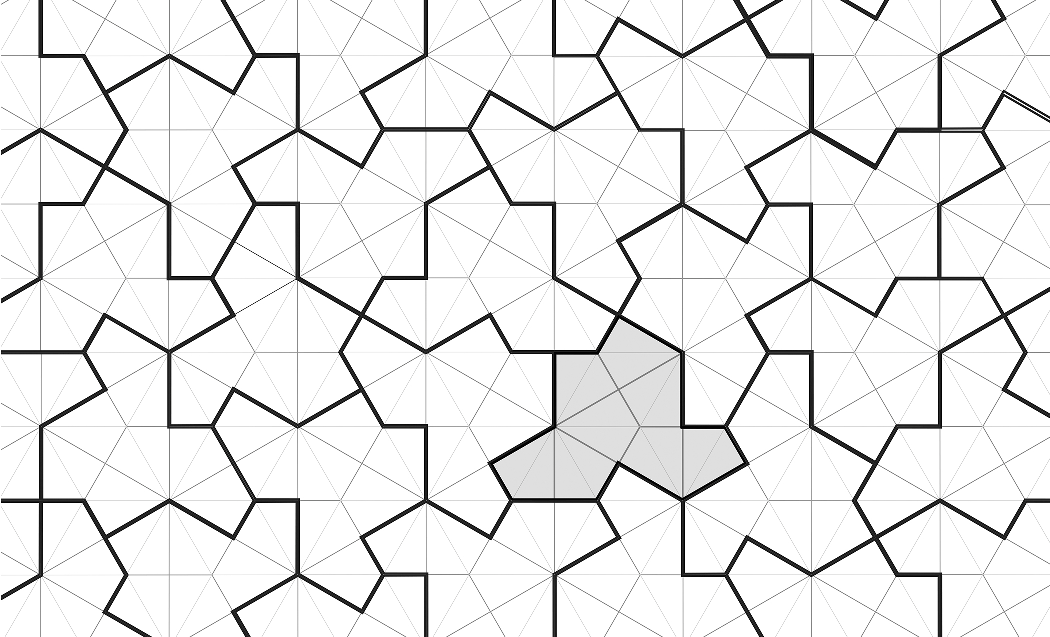
\includegraphics[width=.8\textwidth]{polykite_tiling_raster.pdf}
\end{center}
\caption{\label{fig:polykite} The gray ``hat'' polykite tile
is an ``einstein", an aperiodic monotile. In other words, copies of this tile may be assembled into tilings of the plane (the tile ``admits" tilings), yet copies of the tile cannot form periodic tilings, tilings that have translational symmetry.  In fact, the tile admits uncountably many tilings. In Sections~\ref{sec:substitution},~\ref{sec:clusters}, and~\ref{sec:subst} we describe how these tilings all arise from substitution rules, showing that they all have the same local structure.}
\end{figure}

Given a set of two-dimensional tiles,  the nature of the planar tilings that they admit arises from a deep interaction between the local and the 
global.  Constraints on the ways that pairs of tiles can 
be neighbours determine the structure of an infinite tiling, at all large scales. Constraints encoded in a set of tiles determine the structure of the space of the tilings that it admits, in subtle ways.

{\em Aperiodic} sets of tiles walk a fine line between order and disorder, admitting tilings, but only  those without any translational symmetry, 
never permitting the simple repetition of  periodic tiling.  Their study dates to Wang's work~\cite{Wang} on the then remaining open cases of Hilbert's {\it Entscheidungsproblem}. Wang encoded logical fragments by what are now known as \emph{Wang tiles}, congruent squares with coloured edges, to be
tiled by translation only with colours matching on adjoining edges.
He conjectured that every set of Wang tiles that admits a tiling (possibly
using only a subset of the tiles) must also
admit a periodic tiling, and showed that this would imply the decidability
of the \textit{tiling problem} (or \textit{domino problem}): the question
of whether a given set of Wang tiles admits any tilings at all.
The algorithm would consist of enumerating all possible ways to cover
larger and larger disks.  Eventually one either will run out of ways to
continue, and the tiles do not admit a tiling; or, if there is a fundamental
domain for a periodic tiling, one will eventually discover it. 
If Wang's conjecture held and aperiodic sets of tiles did not exist, this
algorithm would always terminate.

Berger~\cite{Berger} then showed that it was undecidable whether a set
of Wang tiles admits a tiling of the plane. He 
constructed the first aperiodic set of  $20426$~Wang tiles, which he used 
as a kind of scaffolding for encoding finite but unbounded runs of arbitrary computation.

Subsequent decades have spawned a rich literature on aperiodic tiling, touching many  different mathematical and scientific settings---we do not attempt a broad survey here. Yet there remain remarkably few really distinct methods of proving aperiodicity in the plane, despite or due to the underlying undecidability of the tiling problem. 

Berger's initial set comprised thousands of tiles, naturally prompting
the question of how small a set of tiles could be while still forcing
aperiodicity.   
Professional and amateur mathematicians produced successively smaller aperiodic sets, culminating in discoveries by Penrose~\cite{Penrose}
and others of several consisting of just two tiles.  Surveys of these 
sets appear in Chapters~10 and~11 of Gr\"unbaum and Shephard~\cite{GS} and
in an account of the Trilobite and Cross tiles~\cite{ChaimTC}.
A recent table appears in the work of Greenfeld and Tao~\cite{GT1}.

The obvious conclusion of this reduction in size would be to arrive at 
an ``einstein'',\!\footnote{A pun from the German ``ein stein'', roughly ``one 
shape'', popularized by Danzer.} a single shape that tiles aperiodically. 
It has long been an open question whether such a tile exists.  Can one tile 
embody enough complexity to forcibly disrupt  periodic order at all scales?

\subsection{The search for an einstein}

Several candidate tiles have been proposed as einsteins, but they all challenge in some way the concepts
of ``tile'', ``tiling'', or ``aperiodic''.

Gummelt~\cite{Gummelt} and Jeong and Steinhardt~\cite{SteinhardtJeong,JeongSteinhardt}
describe a single regular decagon that can cover the plane with copies that are allowed to overlap by prescribed rules, but only non-periodically, in a manner tightly coupled to the Penrose tiling. 
Senechal~\cite{Senechalpersonalcommunication} similarly describes simple rules that allow copies of the Penrose dart to overlap and cover the plane, but never periodically. The result is an ingenious route to aperiodicity, but not a 
tiling in the usual sense.

The Taylor-Socolar tile~\cite{ST1} comes within a hair's breadth
of being aperiodic.  Their hexagonal prototile tiles
aperiodically, but only when additional matching conditions are enforced, 
preventing certain adjacencies that would otherwise be permitted.
These matching conditions mandate relationships
between non-adjacent tiles, making it impossible to encode 
the global aperiodicity in the shape of a two-dimensional topological
disk.  The matching conditions can be expressed
purely geometrically, but doing so requires either a disconnected tile, a
three-dimensional tile, or one with cutpoints~\cite{ST2}. 

The structure of the Taylor-Socolar
tiling is closely related to Penrose's $1+\epsilon+\epsilon^2$
tiling~\cite{penrose_epsilon}. Like the Trilobite and Crab tiles~\cite{ChaimTC}, these can be adjusted so that an arbitrarily high fraction of the area lies in copies of just one kind of tile, but no matter how thin or small, the other tiles remain  necessary. 

The Schmitt-Conway-Danzer tile~\cite[Section 7.2]{Senechal} tiles
$\mathbb{R}^3$, with tilings that have a screw symmetry but not
translations as symmetries; no periodic tiling by copies of this tile has a compact fundamental domain, and we call this tile \emph{weakly  aperiodic}. Weak aperiodicity  is indeed weak, and readily appears  in the hyperbolic plane and other non-amenable spaces---as early as 1974, B\"or\"oczky exhibited a weakly aperiodic monotile in the hyperbolic plane~\cite{Boroczsky}, the elegantly simple basis of the ``binary tilings''~\cite{BlockWeinberger,regprod,MargulisMozes,Mozes97}.

Following Mozes~\cite{Mozes97}, we say a set of tiles is \emph{strongly aperiodic} if it admits tilings but none with any infinite cyclic symmetry.  In the plane, for  sets of ``normal'' tiles,
these concepts coincide~\cite[Theorem~3.7.1]{GS} and we do not need to make this distinction.

Matching rules for how tiles may fit together have taken many different forms in the literature, and, loosely speaking, it is often possible to shift the complexity in a construction from the tiles to the matching rules or vice versa. For example, if we use a finite atlas of finite configurations as our allowed matching rules, even the lowly $2\times1$ rectangle is an aperiodic monotile!\footnote{Beginning with an aperiodic set of tiles with, say, geometric matching rules, pixelate pictures of the tiles and how they fit together, in some black and white bit-map. Take an atlas of these pictures, splitting black pixels vertically and white ones horizontally into identical rectangles. The rectangle is an aperiodic monotile with this atlas of matching rules.}
The plainest possible rules are just that the tiles must fit together without gaps or overlapping interiors, and these remain the gold standard for an aperiodic monotile.



Moving to higher dimensional space permits richer forms of aperiodicity to
arise.  Recently, Greenfeld and Tao~\cite{GT2} showed that in sufficiently 
high dimensions, a single tile, tiling \emph{only by translation}, can be
aperiodic in~$\mathbb{Z}^n$ (and thus in~$\mathbb{R}^n$).
They also showed that it is undecidable whether a single
tile, again tiling by translation, admits a tiling of a periodic
subset of $\mathbb{Z}^2 \times G$ for some nonabelian group~$G$~\cite{GT1}.
By contrast, in~$\mathbb{R}^2$,
Kenyon~\cite{Kenyon,Kenyonerratum,Kenyon2}, building on the work of
Girault-Beauquier and Nivat~\cite{GiraultBeauquierNivat}, showed that
any topological disk that admits a tiling by translation also admits a
periodic tiling, while Bhattacharya~\cite{Bhattacharya} showed the
same for any set in~$\mathbb{Z}^2$.

Little is known about limits on what sorts of shapes could potentially be
aperiodic monotiles.  Rao~\cite{Rao} showed through a computer
search that the list of 15 known families of convex pentagons that tile the
plane is complete, thereby eliminating any remaining possibility
that a convex polygon could be an einstein.
Jeandel and Rao~\cite{JeandelRao} showed that the smallest aperiodic set
of Wang tiles is of size~$11$.

Even when a single tile admits periodic tilings, that periodicity may be 
more or less abstruse, in a way that offers tantalizing hints about 
aperiodicity.  Here, the \emph{isohedral number} of a tile is the minimum
number of transitivity classes in any tiling it admits; a tile is
\emph{anisohedral} if its isohedral number is greater than one.
The second part of Hilbert's 18th problem~\cite{Hilbert} asked whether
there exist anisohedral polyhedra in $\mathbb{R}^3$. Gr\"unbaum and 
Shephard suggest
\cite[Section~9.6]{GS} that this question was asked in $\mathbb{R}^3$
because Hilbert assumed that no such tiles exist in the plane, yet
Reinhardt~\cite{Reinhardt} found an example of such a polyhedron, and
Heesch~\cite{Heesch} then gave an example of such a tile in the plane.
Many anisohedral prototiles are known today. The computer enumeration
by Myers~\cite{Myers} furnished numerous anisohedral polyominoes, 
polyhexes, and polyiamonds, including a record-holding $16$-hex that
tiles with a minimum of ten transitivity classes.  It is unknown whether
there is an upper bound on isohedral numbers of monotiles.\footnote{The problem of  determining whether or not a given set of tiles admits a periodic tiling is also undecidable, at least for larger sets of tiles~\cite{Gurevich}. If we enumerate sets of tiles, and define $I(n)$ to be the isohedral number of the $n$th set, if it admits a periodic tiling, and let $I(n) = -1$ otherwise, then $I(n)$ cannot be bounded by any computable function. This defies our imagination.}

Related insights can be gleaned from the study of shapes that do not tile
the plane.  A shape's \emph{Heesch number} is the largest possible 
combinatorial radius of any patch formed by copies of the shape (or
equivalently, the maximum number of complete concentric rings that can 
be constructed around it).  A shape that tiles the plane is said to have a
Heesch number of $\infty$.  Heesch first exhibited a shape with Heesch
number~1, and a few isolated examples with Heesch numbers up to three were
discovered thereafter~\cite{Mann2004}.  Mann and Thomas discovered marked
polyforms with Heesch numbers up to~5 through a brute-force computer 
search~\cite{MT2016}.  Kaplan conducted a search on unmarked 
polyforms~\cite{Kaplan}, yielding examples with Heesch numbers up to~4.
Ba{\v{s}}i{\'c} discovered the current record-holder, a shape with Heesch
number~6~\cite{Basic2021}.  \emph{Heesch's problem} asks which 
positive integers can be Heesch numbers; beyond specific examples with
Heesch numbers up to~6, nothing is known about the solution.
An upper bound on finite Heesch numbers would imply the decidability of 
the tiling problem for monotiles. The algorithm would simply consist of
generating all possible concentric rings around a central tile; eventually
you will either fail (in which case the shape does not tile the plane) or
exceed the upper bound on Heesch numbers (in which case it must tile the plane).

\subsection{Outline}

\begin{figure}[htp!]
\begin{center}
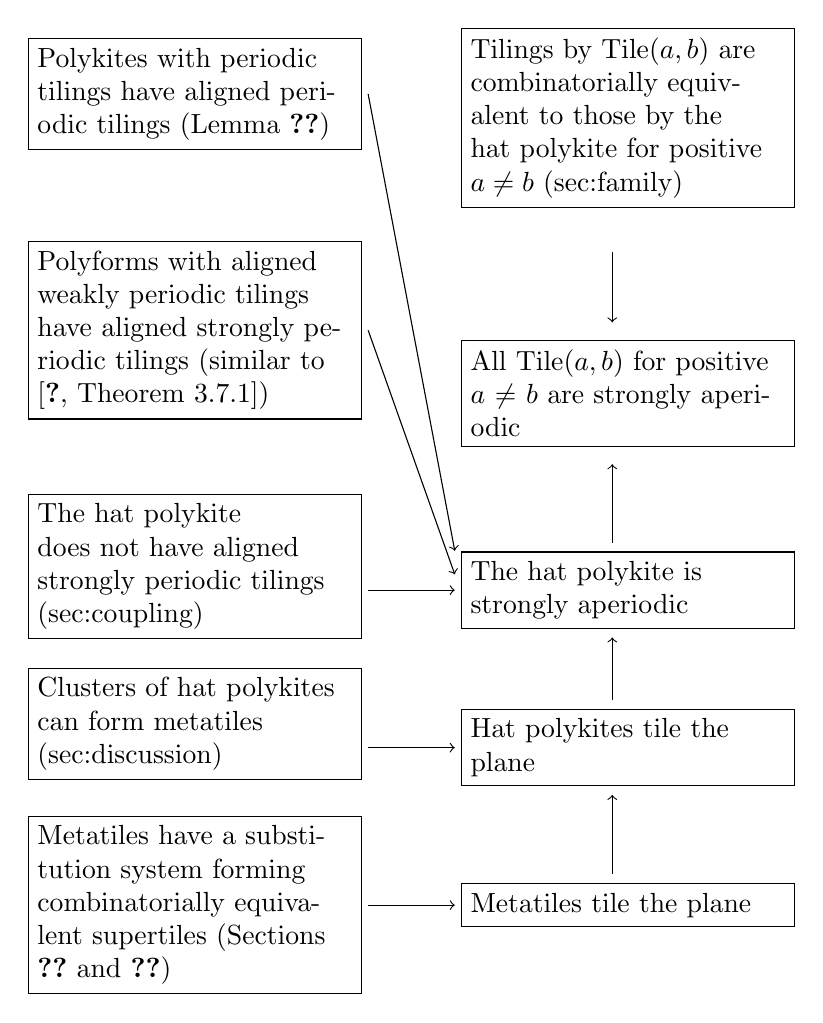
\begin{tikzpicture}[x=1cm,y=1cm]
  \node[draw,text width=4cm] at (0,10.3) {Polykites with periodic tilings
    have aligned periodic tilings (Lemma~\ref{lemma:polykitealign})};
  \node[draw,text width=4cm] at (0,7.3) {Polyforms with aligned weakly
    periodic tilings have aligned strongly periodic tilings (similar
    to \cite[Theorem~3.7.1]{GS})};
  \node[draw,text width=4cm] at (0,4.3) {The hat polykite does not have
    aligned strongly periodic tilings (\secref{sec:coupling})};
  \node[draw,text width=4cm] at (0,2.3) {Clusters of hat polykites can form
    metatiles (\secref{sec:discussion})};
  \node[draw,text width=4cm] at (0,0) {Metatiles have a substitution
    system forming combinatorially equivalent supertiles
    (Sections \ref{sec:discussion} and~\ref{sec:subst})};
  \node[draw,text width=4cm] at (5.5,0) {Metatiles tile the plane};
  \node[draw,text width=4cm] at (5.5,2) {Hat polykites tile the plane};
  \node[draw,text width=4cm] at (5.5,4) {The hat polykite is strongly
    aperiodic};
  \node[draw,text width=4cm] at (5.5,6.5) {All $\mathrm{Tile}(a, b)$ for
    positive $a \ne b$ are strongly aperiodic};
  \node[draw,text width=4cm] at (5.5,10) {Tilings by $\mathrm{Tile}(a,b)$ are
    combinatorially equivalent to those by the hat polykite for
    positive $a \ne b$ (\secref{sec:family})};
  \draw[->] (2.2,0) -- (3.3,0);
  \draw[->] (2.2,2) -- (3.3,2);
  \draw[->] (2.2,4) -- (3.3,4);
  \draw[->] (2.2,7.3) -- (3.3,4.2);
  \draw[->] (2.2,10.3) -- (3.3,4.5);
  \draw[->] (5.3,0.4) -- (5.3,1.4);
  \draw[->] (5.3,2.6) -- (5.3,3.4);
  \draw[->] (5.3,4.6) -- (5.3,5.6);
  \draw[->] (5.3,8.3) -- (5.3,7.4);
\end{tikzpicture}
\end{center}
\caption{The high-level structure of the first proof of aperiodicity in
  this paper}
\label{fig:proofstructure}
\end{figure}

\begin{figure}[ht!]
\begin{center}
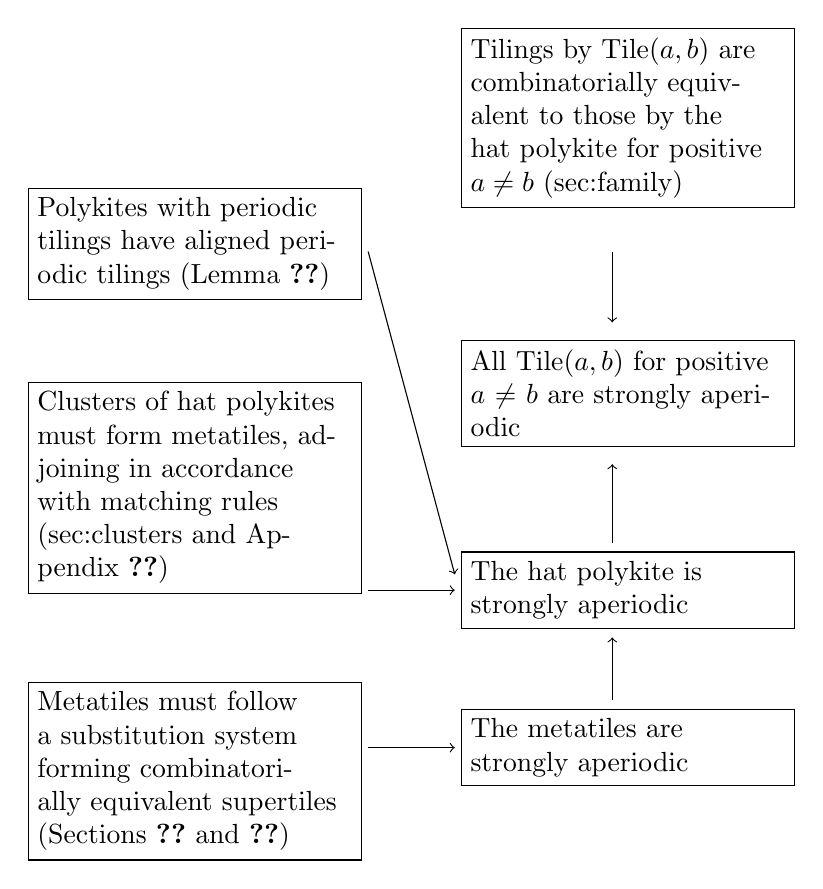
\begin{tikzpicture}[x=1cm,y=1cm]
  \node[draw,text width=4cm] at (0,6.4) {Polykites with periodic tilings
    have aligned periodic tilings (Lemma~\ref{lemma:polykitealign})};
  \node[draw,text width=4cm] at (0,3.3) {Clusters of hat polykites
    must form metatiles, adjoining in accordance with matching rules
    (\secref{sec:clusters} and Appendix~\ref{sec:patches})};
  \node[draw,text width=4cm] at (0,-0.3) {Metatiles must follow a
    substitution system forming combinatorially equivalent supertiles
    (Sections \ref{sec:discussion} and~\ref{sec:subst})};
  \node[draw,text width=4cm] at (5.5,0) {The metatiles are strongly aperiodic};
  \node[draw,text width=4cm] at (5.5,2) {The hat polykite is strongly
    aperiodic};
  \node[draw,text width=4cm] at (5.5,4.5) {All $\mathrm{Tile}(a, b)$ for
    positive $a \ne b$ are strongly aperiodic};
  \node[draw,text width=4cm] at (5.5,8) {Tilings by $\mathrm{Tile}(a,b)$ are
    combinatorially equivalent to those by the hat polykite for
    positive $a \ne b$ (\secref{sec:family})};
  \draw[->] (2.2,0) -- (3.3,0);
  \draw[->] (2.2,2) -- (3.3,2);
  \draw[->] (2.2,6.3) -- (3.3,2.2);
  \draw[->] (5.3,0.6) -- (5.3,1.4);
  \draw[->] (5.3,2.6) -- (5.3,3.6);
  \draw[->] (5.3,6.3) -- (5.3,5.4);
\end{tikzpicture}
\end{center}
\caption{The high-level structure of the second proof of aperiodicity in
  this paper}
\label{fig:proofstructure2}
\end{figure}

In this paper, we prove the following:  

\begin{theorem}
\label{thm:main}
The shape shown shaded in \fig{fig:polykite}, a polykite that we call
``the hat'', is an aperiodic monotile.
\end{theorem}

No special qualifications or additional
matching conditions are required: as shown, this shape tiles the plane,
but never with any translational symmetries.
The shape is almost mundane in its simplicity. It is a \textit{polykite}:
the union of eight kites in the Laves tiling $[3.4.6.4]$, the dual to the 
$(3.4.6.4)$ Archimedean tiling.

We provide two different proofs of aperiodicity, both with novel
aspects.  The first proof follows the structure shown in
\fig{fig:proofstructure}, centred on a 
new approach in \secref{sec:coupling} for proving aperiodicity in the plane.
We observe that
any tiling by the hat corresponds to tilings by two different
polyiamonds, one with twice the area of the other.  If there were a
strongly periodic tiling by the hat, the other two tilings would also
be strongly periodic. We prove that if so, the lattices of
translations in the polyiamond tilings would necessarily be related by a
similarity; but
no similarity between lattices of translations on the regular
triangular tiling can have the scale factor~$\sqrt{2}$ required by the
ratio of the areas.  This does not show that a tiling exists, and so
must be combined with an explicit construction of a tiling (outlined
in \secref{sec:discussion} and given in detail in Sections
\ref{sec:clusters} and~\ref{sec:subst}) to complete the proof of
aperiodicity.

The second proof presented (but the first one found) follows the structure
shown in \fig{fig:proofstructure2}.  Here we generally adhere to
Berger's approach, but we must begin with a novel step
to get to the point where such a proof is possible.  
We first show that in any tiling by
the hat polykite, every tile belongs uniquely to one of four distinct
clusters (\secref{sec:clusters}), and that those clusters fit together
following certain matching rules.
It is then the clusters that allow a more standard style of 
hierarchical construction.
This  remarkable behaviour has not been seen previously in the literature.

Defining matching rules on the boundaries of the clusters allows us to
discard details of how the clusters are made up of hats, and instead
consider simplified outlines we refer to as \emph{metatiles}.
Following Berger et al., we then give an inductive proof in \secref{sec:subst}
showing that any
tile in any tiling by these four metatiles lies in a unique hierarchy
of larger and larger \textit{supertiles}, effectively combinatorial copies
of the metatiles, at larger and larger scales. The proof is
constructive: we first show the metatiles can only lie within larger
clusters, the $1$-level supertiles, uniquely, and that these clusters
have the same combinatorial structure as the metatiles. In turn, in
the same manner, the $1$-level supertiles can only lie uniquely within
$2$-level supertiles, again clusters with the same combinatorics, and so on
for subsequent levels.
This construction proves that tilings by copies of the
metatiles can only be non-periodic, because if there were a
translational symmetry, these hierarchies of supertiles could not be
unique. It also shows that the metatiles (and hence the hats) admit 
tilings of the plane, because we
construct clusters of arbitrary size~\cite[Theorem 3.8.1]{GS}.

Because of the combinatorial complexity of the hat polykite, 
a significant fraction of our second proof relies on exhaustive enumeration
of cases, which we carried out and cross-checked with two 
independent software implementations developed by two of the authors
in isolation.  These calculations are necessarily ad hoc, and are essentially
unenlightening.  This case
analysis is only needed to show that all tilings follow the
substitution structure; it is not needed for showing that a tiling
exists, and thus is not needed to show that the tile is aperiodic,
given the proof in \secref{sec:coupling} that no periodic tiling exists.

We close this introduction with definitions of the essential terminology
we will need for the rest of the article.
In \secref{sec:discussion},
we then present a compendium of provisional observations about this polykite,
including an explicit construction of a tiling and aspects of its structure
that deserve further study.  Our two proofs of aperiodicity follow:
we show that there are no periodic tilings (\secref{sec:coupling}),
then that tiles must group into clusters that define metatiles
equipped with matching rules (\secref{sec:clusters}),
and finally that metatiles must compose into
supertiles with combinatorially equivalent matching rules
(\secref{sec:subst}).
In \secref{sec:family}, we offer additional remarks about the continuum
of tiles that contains the hat polykite.  As noted there,
computer search shows that the hat is the smallest aperiodic polykite.

\subsection{Terminology}
\label{sec:terminology}

Terminology used for tilings generally follows that of
Gr\"unbaum and Shephard~\cite{GS}.

A \emph{tile} in a metric space is a closed set of points from that
space. A \emph{tiling} by a set of tiles is a collection of images of
tiles from that set under isometries, the interiors of which are
pairwise disjoint and the union of which is the whole space; we
say a set of tiles \emph{admits} the tiling, or in the case of a single tile
that it admits the tiling.  For most purposes, it is convenient for
tiles to be nonempty compact sets that are the closures of their
interiors; the tiles considered here are polygons, or more generally
closed topological disks.  A
tiling is \emph{monohedral} if all its tiles are congruent.  All
tilings considered here are also \emph{locally finite}: every point
has some open neighbourhood that meets only finitely many tiles (all
monohedral plane tilings by closed topological disks are locally
finite).

In any locally finite tiling of the plane by closed topological disks,
the connected components of the intersection of two or more tiles are
isolated points, which are called \emph{vertices} of the tiling, and
Jordan arcs, which are called \emph{edges} of the tiling, and the
boundary of any tile is divided into finitely many edges, alternating
with vertices. Each edge lies on the boundary of exactly two tiles,
which we refer to as lying on opposite sides of the edge.  Two
distinct tiles are \emph{neighbours} if they share any point of their
boundaries, and \emph{adjacents} if they share an edge.

When a (closed topological disk) tile has a polygonal boundary, we
refer to it as having \emph{sides} (maximal straight line segments
lying on that boundary) and \emph{corners} (between two sides), to
distinguish from the edges and vertices of a tiling.  We rely on
context to distinguish the meanings of ``side'' as referring to sides
of a polygon or the two sides of an edge of a tiling.  A tiling by
polygons is \emph{edge-to-edge} if the corners and sides of the
polygons coincide with the vertices and edges of the tiling.

A \textit{patch} of tiles is a collection of non-overlapping tiles whose
union is a topological disk.  More specifically, a \textit{$0$-patch}
is a patch containing a single tile, and an \textit{$(n+1)$-patch} is 
a patch formed from the union of an $n$-patch $P$ and a set $S$ of
additional tiles, so that $P$ lies in the interior of the patch and no
proper subset of~$S$ yields a patch with $P$ in its interior.  (In
other words, an $(n+1)$-patch is
a tile surrounded by $n$ concentric rings of tiles.)  In a fixed tiling,
every tile generates an $n$-patch for all finite $n$, by recursively
constructing an $(n-1)$-patch and adjoining all its neighbours in the
tiling, along with any other tiles required to fill in holes left by
adding neighbours.

Given a tiling~$\mathcal{T}$, a \emph{poly-$\mathcal{T}$-tile} is a
closed topological disk that is the union of finitely many tiles
from~$\mathcal{T}$. Poly-$\mathcal{T}$-tiles are also referred to
generically as \emph{polyforms}.  Poly-$\mathcal{T}$-tiles may also
be defined so that they are permitted to have holes.
Because we are mainly concerned with tiles
that admit monohedral tilings, it is not generally significant for the
purposes of this paper whether shapes with holes are allowed or not.

The \emph{symmetry group} of a tiling is the group of those isometries
that act as a permutation on the tiles of the tiling.  A tiling is
\emph{weakly periodic} if its symmetry group has an element of
infinite order; in the plane, this means it includes a nonzero
translation.  A tiling is \emph{strongly periodic} if the symmetry
group has a discrete subgroup with cocompact action on the space
tiled. In Euclidean space, all strongly periodic
tilings are also weakly periodic.  A set of tiles (or a single tile)
is \emph{weakly aperiodic} if it admits a tiling but does not admit a
strongly periodic tiling, and \emph{strongly aperiodic} if it admits a
tiling but does not admit a weakly periodic tiling.

Any finite set of polygons in the plane that admits a weakly periodic
edge-to-edge tiling also admits a strongly periodic
tiling~\cite[Theorem~3.7.1]{GS}, and a similar but simpler argument
shows the same to be the case for a finite set of
poly-$\mathcal{T}$-tiles where $\mathcal{T}$ is itself a strongly
periodic tiling and the weakly periodic tiling consists of copies 
of the
tiles all aligned to the same underlying copy of~$\mathcal{T}$,
instead of being edge-to-edge.  Thus in such contexts it is not
necessary to distinguish weak and strong aperiodicity and we refer to
tiles and sets of tiles simply as \emph{aperiodic}.

A \emph{uniform tiling}~\cite[Section~2.1]{GS} is an edge-to-edge
tiling by regular polygons with vertex-transitive symmetry group;
notation such as $(3.4.6.4)$, listing the sequence of regular polygons
round each vertex, denotes a uniform tiling.  A \emph{Laves
tiling}~\cite[Section~2.7]{GS} is an edge-to-edge monohedral tiling by
convex polygons with regular vertices (all angles between consecutive
edges at a vertex equal) and tile-transitive symmetry group; analogous
notation such as $[3.4.6.4]$ is used for Laves tilings, listing the
sequence of vertex degrees round each tile, and in an appropriate
sense Laves tilings are dual to uniform tilings.
